
\documentclass[conference]{IEEEtran}
\IEEEoverridecommandlockouts

%% ==========================================
%%   ECE 50874/59500 - FINAL REPORT TEMPLATE
%%          TRACK: ENGINEERING
%% ==========================================

%% ==========================================
%% 1. PACKAGES
%% ==========================================
\usepackage{cite}
\usepackage{amsmath,amssymb,amsfonts}
\usepackage{algorithmic}
\usepackage{graphicx}
\usepackage{textcomp}
\usepackage{xcolor}
\usepackage{float}
\usepackage{url}
\usepackage[colorlinks=true, urlcolor=blue, linkcolor=blue]{hyperref}

% BibTeX
\def\BibTeX{{\rm B\kern-.05em{\sc i\kern-.025em b}\kern-.08em
    T\kern-.1667em\lower.7ex\hbox{E}\kern-.125emX}}

%% ==========================================
%% 2. INSTRUCTION COMMAND
%% ==========================================
\newcommand{\instruction}[1]{%
    \begin{list}{}{%
        \leftmargin=10pt
        \rightmargin=10pt
        \topsep=0.5em
    }
    \item[]
    \begingroup
        \color{gray}\itshape
        \small
        
        \textbf{Instructions:} #1
    \endgroup
    \end{list}
}

\begin{document}

%% ==========================================
%% 3. TITLE & AUTHORS
%% ==========================================
\title{Design and Evaluation of a Cost-Aware Runtime for OpenClaw Browser Agents\\
}

% Authors
\author{\IEEEauthorblockN{1\textsuperscript{st} W. Spencer Darby}
\IEEEauthorblockA{\textit{ECE Department} \\
\textit{Purdue University}\\
Phoenix, Arizona, United States of America \\
darbyw@purdue.edu}
\and
\IEEEauthorblockN{2\textsuperscript{nd} Ming Jia}
\IEEEauthorblockA{\textit{ECE Department} \\
\textit{Purdue University}\\
Los Angeles, California, United States of America \\
jia213@purdue.edu}
\and
\IEEEauthorblockN{3\textsuperscript{rd} Dovid Korn}
\IEEEauthorblockA{\textit{ECE Department} \\
\textit{Purdue University}\\
New Orleans, Louisiana, United States of America \\
korn4@purdue.edu}
\and
\IEEEauthorblockN{4\textsuperscript{th} Ian Nicholas Karlmann}
\IEEEauthorblockA{\textit{ECE Department} \\
\textit{Purdue University}\\
Los Angeles, California, United States of America \\
ikarlman@purdue.edu}
}

\maketitle

%% ==========================================
%% 4. BODY
%% ==========================================

\begin{abstract}
\instruction{You must use a \textbf{STRUCTURED ABSTRACT}. Do not write a single block of text.
Follow the specific headings (Context, Objective, Method, Results, Conclusion) defined in the guidelines:
\begin{itemize}
    \item Guidelines: \href{https://link.springer.com/journal/10664/submission-guidelines}{Springer Submission Guidelines}
    \item Reference Example: \href{https://link.springer.com/article/10.1007/s10664-024-10521-0}{Example Article (Springer)}
\end{itemize}}
\end{abstract}

\begin{IEEEkeywords}
implementation, software engineering, system design
\end{IEEEkeywords}

\section{Introduction}

Browser-based AI agents are increasingly used to automate tasks that require direct interaction with web applications, including form completion, information retrieval, and navigation of complex user interfaces. Frameworks such as OpenClaw support this capability by combining large language model reasoning with browser automation, enabling agents to observe page state and execute actions such as clicks, text input, and navigation.

In practice, however, controlling browser-based agents remains challenging. Modern web applications rely heavily on asynchronous loading, dynamic content updates, and deeply nested DOM structures, all of which can interfere with an agent’s ability to reason effectively about page state. When an agent encounters unexpected or ambiguous behavior, it may repeatedly attempt similar actions without making progress. These execution loops increase token usage, incur unnecessary API cost, and introduce additional latency, often without providing clear feedback to the user until execution has completed.

This project investigates an alternative approach in which execution cost and performance awareness are embedded directly into the agent runtime. Rather than treating cost as a post-hoc metric, we integrate a cost-aware execution layer into OpenClaw using the AgentOps framework. By monitoring metrics such as cost per action, latency trends, and task progress during execution, the runtime can intervene before budgets are exhausted or execution quality degrades. The remainder of this paper describes the design of this integration and presents an evaluation strategy for assessing its effectiveness in controlling runaway execution while preserving task success.


\section{Background and Related Work}

This project builds on prior work in browser-based AI agents and execution monitoring frameworks. While recent systems have focused on improving agent autonomy and task capability, comparatively less attention has been given to governing execution behavior once an agent is deployed. This section reviews relevant browser-agent architectures and execution governance tools, with particular emphasis on OpenClaw and AgentOps.

\subsection{Browser-Based Agent Architectures}

Browser-based agents extend large language models by allowing them to perceive and manipulate web interfaces through automated browsers. OpenClaw is a representative open-source framework that follows this paradigm, providing a modular architecture that separates agent reasoning, browser state observation, and action execution \cite{openclaw}. This separation enables agents to iteratively observe page state, select an action, and execute browser interactions such as clicks, text input, or navigation.

While this architecture provides flexibility, OpenClaw does not natively account for execution cost or latency during runtime. Browser actions are executed without explicit awareness of cumulative token usage, per-action latency, or task-level budget constraints. As a result, when agents encounter dynamic or unexpected page structures, they may repeatedly execute ineffective actions without detection. Prior work on reasoning-and-acting agents has shown that such execution patterns are common in complex environments, particularly when agents rely on partial or noisy observations \cite{yao2022react}.

\subsection{Execution Monitoring and Governance Frameworks}

AgentOps is an open-source framework designed to provide observability into agent execution by tracking metrics such as token usage, cost, and execution traces \cite{agentops}. These capabilities support debugging and post-hoc analysis but are typically applied alongside agent frameworks rather than integrated directly into the execution loop.

Related tools such as LangGraph introduce structured execution graphs that improve reasoning transparency but do not enforce execution budgets at runtime \cite{langgraph}. From a software engineering perspective, this separation between execution and governance contrasts with established principles of resource-aware system design, where monitoring and enforcement are tightly coupled with execution.

The SIGSOFT Empirical Standards emphasize the importance of clearly defined measurement boundaries, construct validity, and alignment between observed metrics and system behavior \cite{sigsoft2020standards}. Applying these principles to browser-based agents suggests that execution metrics such as cost per action and latency should be collected and evaluated at the same abstraction level at which actions are executed. This project addresses this gap by integrating AgentOps directly into OpenClaw’s browser-action execution layer.



\section{Problem Statement}

Browser-use agents frequently exhibit runaway execution behavior when interacting with complex or unexpected web interfaces. Existing frameworks, including OpenClaw, prioritize agent autonomy and task completion but provide limited mechanisms for enforcing execution budgets or detecting ineffective action patterns during runtime.

\section{Problem Statement}

Browser-based agents frequently exhibit runaway execution behavior when interacting with complex or unexpected web interfaces. Although frameworks such as OpenClaw prioritize agent autonomy and task completion, they provide limited mechanisms for detecting ineffective behavior or enforcing execution budgets during runtime.

\subsection{Goals and Requirements}

The primary goal of this project is to prevent uncontrolled execution while maintaining the flexibility and generality of browser-based agents. Specifically, the system is designed to:
\begin{itemize}
    \item Prevent runaway execution loops during browser interaction.
    \item Enforce cost, latency, and execution-step budgets at runtime.
    \item Detect degradation in agent performance using measurable execution signals.
    \item Enable proactive intervention without modifying core agent logic.
\end{itemize}

To achieve these goals, the system must support real-time tracking of cost per action, latency, and task progress. Intervention policies, such as early termination or strategy adjustment, must be configurable while imposing minimal overhead and remaining compatible with existing OpenClaw workflows.

\subsection{Gap Analysis}

Existing browser-agent frameworks provide robust abstractions for browser interaction but lack integrated execution governance. While AgentOps offers detailed observability into agent behavior, it does not intervene during execution when used as a standalone tool. The proposed integration addresses this limitation by embedding monitoring and enforcement directly into the agent runtime, closing the gap between execution and governance.
\begin{table}[h]
\centering
\caption{Comparison of Browser-Agent Execution Capabilities}
\label{tab:gap}
\begin{tabular}{lccc}
\hline
\textbf{System} & \textbf{Budget Enforcement} & \textbf{Telemetry} & \textbf{Intervention} \\
\hline
OpenClaw (baseline) & X & X & X \\
AgentOps (standalone) & \checkmark & \checkmark & X \\
Proposed Integration & \checkmark & \checkmark & \checkmark \\
\hline
\end{tabular}
\end{table}

\section{System Design / Implementation}
\instruction{\textbf{Core Section.} Describe your solution architecture.
\begin{itemize}
    \item Explain the system architecture and design choices.
                \item Detail the implementation steps and technologies used.
\item \textbf{Visual Requirement:} Include diagrams of the system flow or components (at least one figure is mandatory).
\end{itemize}}
\begin{figure}
        \centering
        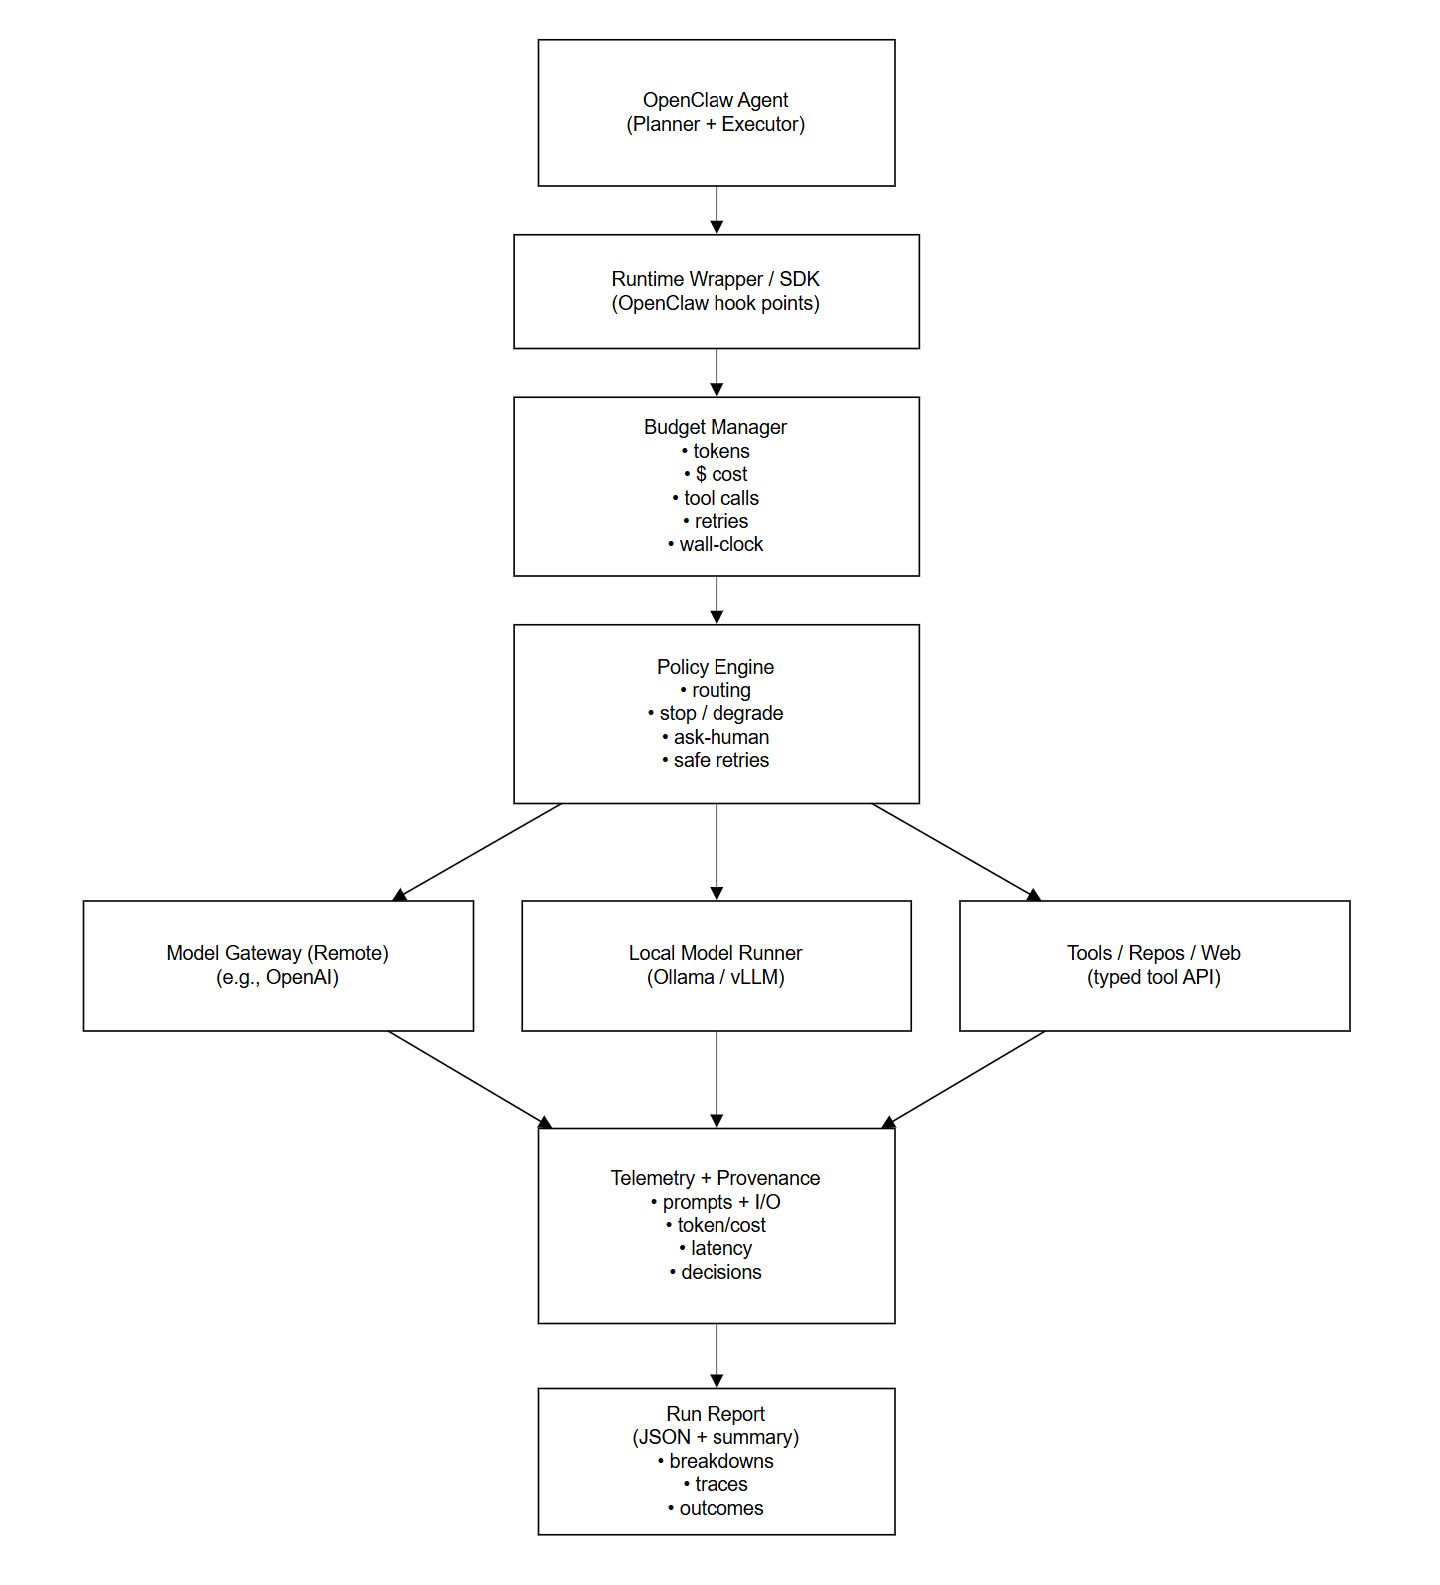
\includegraphics[width=0.5\linewidth]{system_architecture.png}
        \caption{System Architecture}
        \label{fig:system_architecture}
    \end{figure}
\begin{figure}
        \centering
        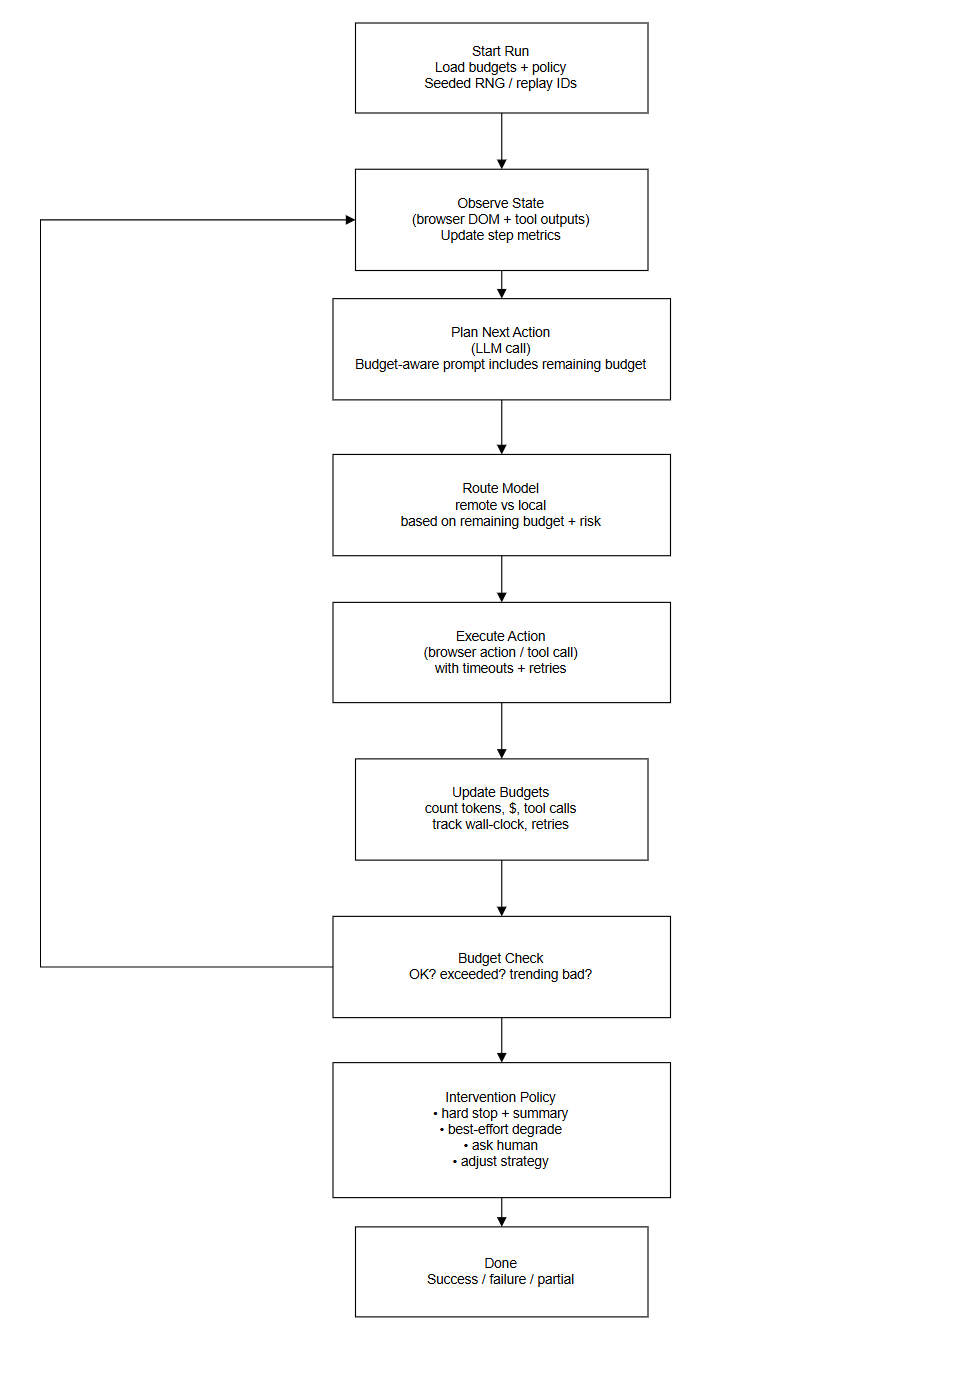
\includegraphics[width=0.5\linewidth]{agent_loop.png}
        \caption{Agent Loop}
        \label{fig:agent_loop}
    \end{figure}
\begin{figure}
        \centering
        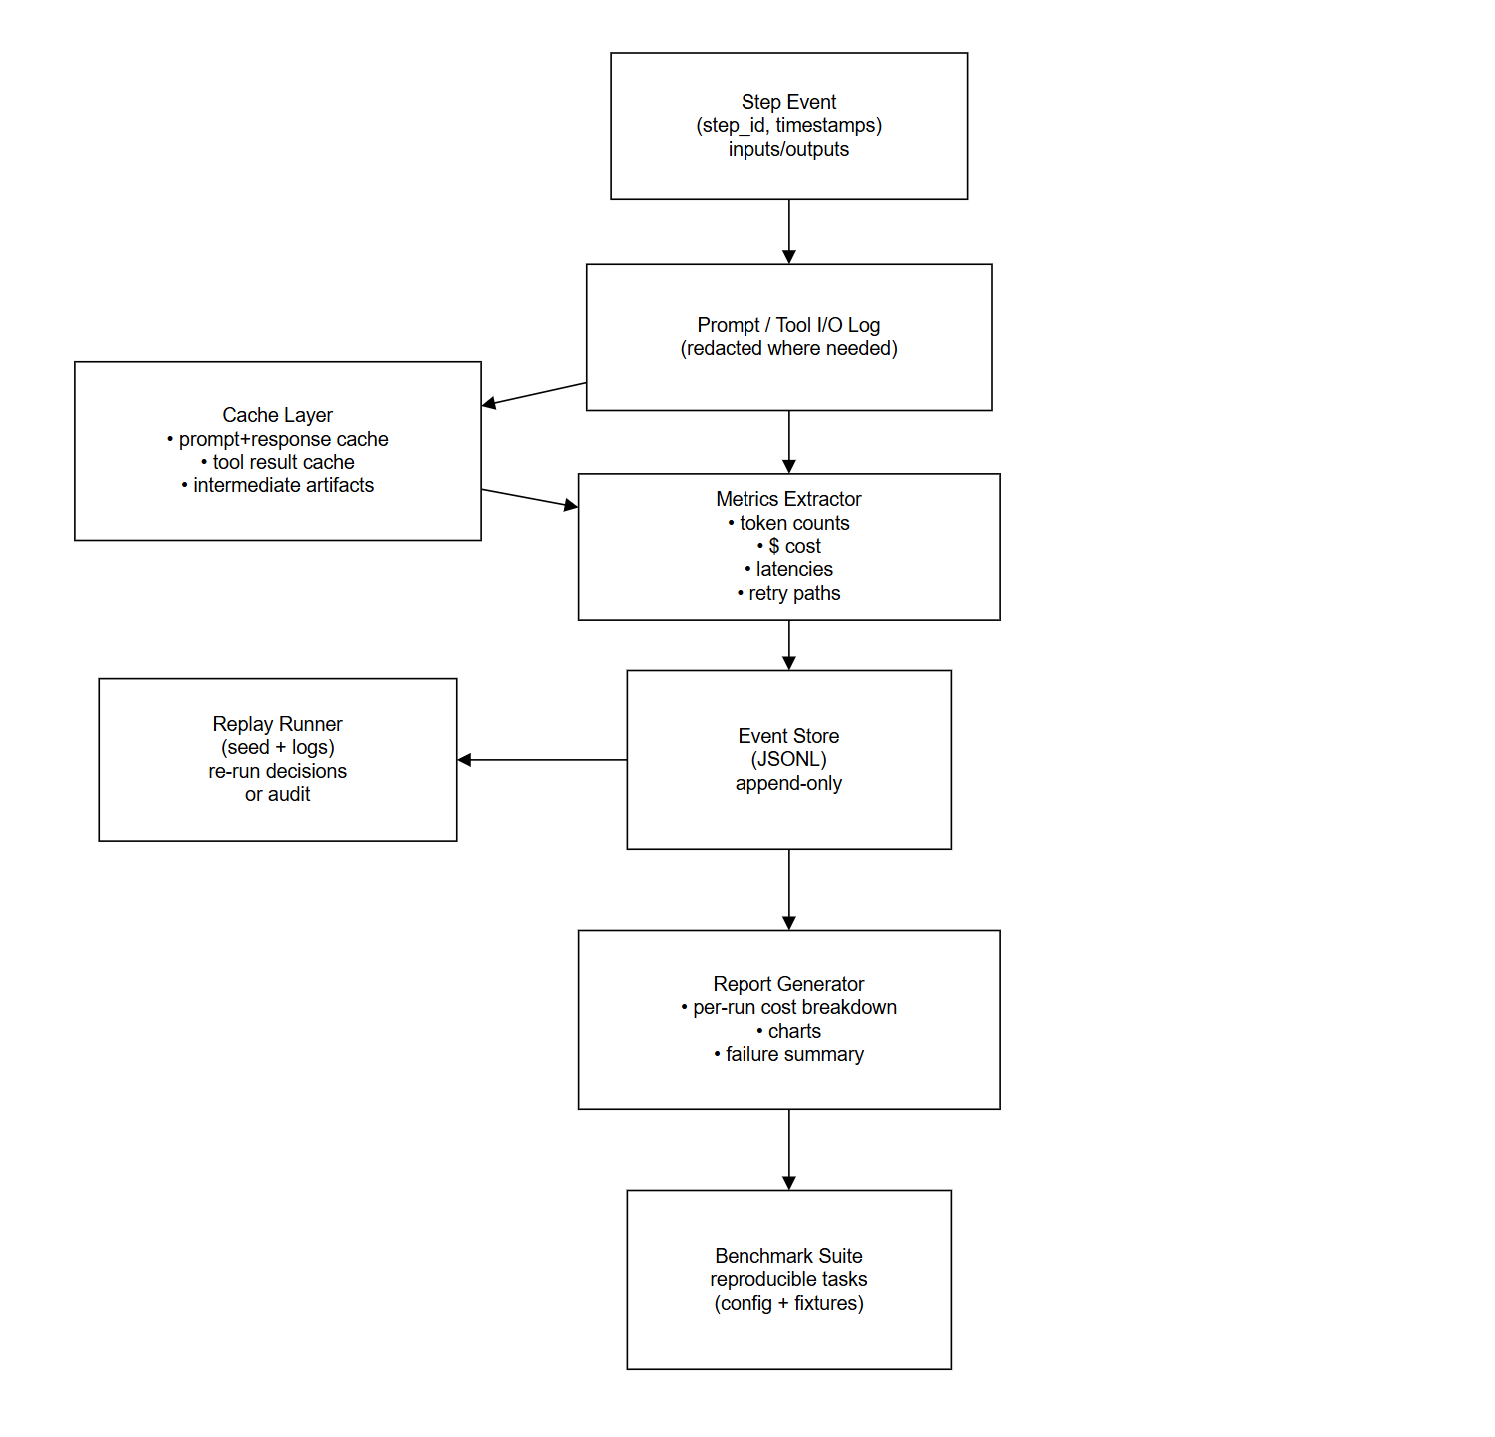
\includegraphics[width=0.5\linewidth]{data_management.png}
        \caption{Data Management}
        \label{fig:data_management}
    \end{figure}
\section{Evaluation and Results}
\instruction{How was the system tested or validated?
\begin{itemize}
    \item Describe your testing strategy (Unit tests, Integration tests, User studies).
    \item Present performance metrics or validation results.
    \item Demonstrate that the Engineering Goals were met.
\end{itemize}}

\section{Analysis and Discussion}
\instruction{Interpret the findings.
\begin{itemize}
    \item Discuss the constraints and trade-offs encountered during implementation.
    \item Discuss limitations of the current solution.
\end{itemize}}

\section{Limitations}
\instruction{Discuss potential issues or boundaries of your solution.
\begin{itemize}
    \item \textbf{Deep Analysis:} Apply Ousterhout's principle ``Always Measure One Level Deeper'' to explain behavior. Refer: \href{https://dl.acm.org/doi/10.1145/3213770}{Ousterhout's Paper}
    \item \textbf{Construct Validity:} Discuss whether you are measuring what you intend to measure. Refer: \href{https://dl.acm.org/doi/10.1145/3530019.3530020}{Verdecchia et al. Analysis}
    \item \textbf{Technical Constraints:} In what real-world scenarios does the solution fail?
\end{itemize}}

\section{Conclusion}
\instruction{Summarize the achievements and suggest future work.}

\section*{Acknowledgment}
\instruction{Acknowledge any help or resources.}

%% ==========================================
%% 5. REFERENCES
%% ==========================================
\bibliographystyle{IEEEtran}
\bibliography{refs} 

%% ==========================================
%% 6. APPENDICES (Process Reflection)
%% ==========================================
\appendices

\section{Project Artifacts}
\instruction{Link to the GitHub repo, datasets, or tools produced. Provide brief descriptions.}

\section{Project Postmortem}

\subsection{Process \& Outcomes Reflection}
\instruction{Compare proposed vs. actual process and outcomes. What changed and why?}

\subsection{Team Retrospective}
\instruction{What went well? What went poorly? (Process-focused).}

\end{document}